\documentclass{article}

\usepackage[french]{babel}
\usepackage[utf8]{inputenc}
\usepackage{graphicx}
\usepackage{amssymb, amsmath, amsthm}

%%%%%%%%%%%%%%%% Lengths %%%%%%%%%%%%%%%%
\setlength{\textwidth}{15.5cm}
\setlength{\evensidemargin}{0.5cm}
\setlength{\oddsidemargin}{0.5cm}

%%%%%%%%%%%%%%%% Variables %%%%%%%%%%%%%%%%
\def\projet{4}
\def\titre{Systèmes d'équations non linéaires / Méthode de Newton-Raphson}
\def\groupe{4}
\def\equipe{1}
\def\responsible{}
\def\secretary{}
\def\others{}

\begin{document}

%%%%%%%%%%%%%%%% Header %%%%%%%%%%%%%%%%
\noindent\begin{minipage}{0.98\textwidth}
  \vskip 0mm
  \noindent
  { \begin{tabular}{p{7.5cm}}
      {\bfseries \sffamily
        Projet \projet} \\ 
      {\itshape \titre}
    \end{tabular}}
  \hfill 
  \fbox{\begin{tabular}{l}
      {~\hfill \bfseries \sffamily Groupe \groupe\ - Equipe \equipe
        \hfill~} \\[2mm] 
      Responsable : \responsible \\
      Secrétaire : \secretary \\
      Codeurs : \others
    \end{tabular}}
  \vskip 4mm ~

  ~~~\parbox{0.95\textwidth}{\small \textit{Résumé~:} \sffamily
    Ce projet a pour but de calculer la(les) racine(s) d'un système d'equations non-linéaires. La méthode proposée ici est celle de Newton-Raphson.
    L'objectif est d'évaluer les avantages et les inconvénients d'une telle solution.
    Cela sera fait en testant la méthode dans différents contextes.
  }
  \vskip 1mm ~
\end{minipage}

%%%%%%%%%%%%%%%% Main part %%%%%%%%%%%%%%%%

\section{Méthode de Newton-Raphson}
Dans cette partie, la méthode de Newton-Raphson a été implémentée pour résoudre un système d'équations non linéaires. Cette méthode permet de donner une approximation de la racine de l'équation, qu'il s'agisse d'une équation unidimensionnelle ou multidimensionnelle.

\subsection{Newton-Raphson standard}
Soit $f : \mathbb{R}^n \to \mathbb{R}^n$ définie comme suit :


fonction ici


La jacobienne de cette fonction est la matrice des dérivées partielles selon chaque variable de cette fonction.


jacobienne ici


Le principe de la méthode peut être résumé comme suit :
\begin{itemize}
\item Étant donné un vecteur initial $U_0$, il faut trouver un vecteur $U$ tel que pour tout $\epsilon$ petit $ |f(U)| \le \epsilon $.
\end{itemize}

Pour trouver ce vecteur, l'algorithme doit trouver un vecteur $V$ qu'il faut ajouter au vecteur $U$
pour approcher $f(U+V)$ de $0$.
Il est possible de remplacer $f(U+V)$ par $f(U) + J(U) \cdot V$, ainsi il faut résoudre l'équation $J(U) \cdot H = -f(U)$.
Ceci va être fait en utilisant la fonction \emph{numpy.linalg.lstsq}.

Ce processus sera répété au plus $N_{max}$ fois.
On peut donc conclure que cet algorithme est de complexité $O(N_{max} \times c)$ avec c la complexité de \emph{numpy.linalg.lstsq}.

\subsection{Newton-Raphson avec du backtracking}
La méthode de Newton-Raphson permet bien de trouver la racine, mais pas dans tous les cas, voir figure~\ref{fig:p1-cvg},
c'est pour cela qu'on va utiliser une méthode nommée du backtracking qui permet d'améliorer la
convergence vers cette racine.
Pour ceci, on ajoute des lignes de code qui permettent de vérifier si la condition
$|f(U + \alpha \times V)|\le|f(U)|$ est vérifiée ou pas. On a essayé de diviser $\alpha$ par deux à chaque
itération mais on a rapidement remarqué que la convergence n'est pas assurée. On a donc dû diviser
$\alpha$ par $1.1$.


Pour conclure, on remarque bien que Newton-Raphson avec du backtracking converge vers la racine
contrairement à celle standard selon la figure~\ref{fig:p1-cvg}.
\begin{figure}[htbp]
\centering
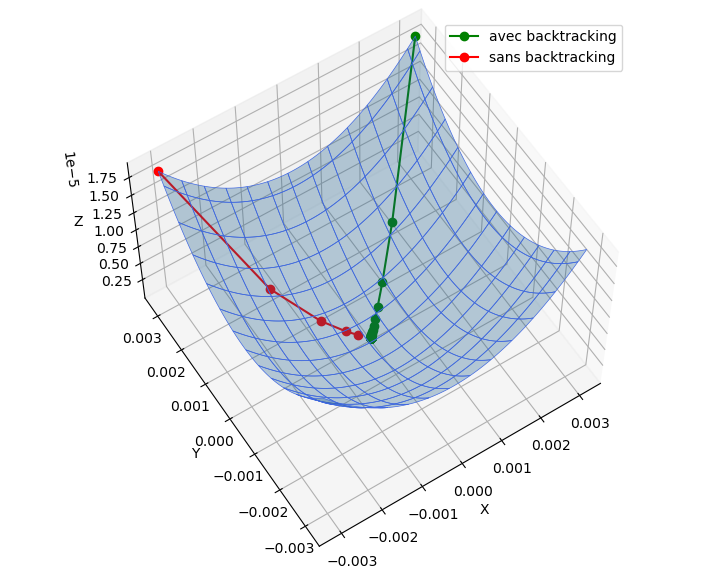
\includegraphics[width=0.65\textwidth]{res/fast_convergence_bt.png}
\caption{Newton-Raphson avec et sans backtracking}
\label{fig:p1-cvg}
\end{figure}
Mais ceci nous coûte en complexité puisque la complexité de Newton-Raphson avec du backtracking
est égale à $O(a \times N_{max} \times c)$ avec c la complexité de \emph{numpy.linalg.lstsq}.\label{sec1}

\section{Les points de Lagrange}
Le but de cette partie est de trouver le point d'équilibre d'un objet sachant qu'il est soumis à plusieurs forces différentes.

\subsection{Modélisation de différentes forces}
Il a donc fallu dans un premier écrire des algorithmes qui vont permettre de calculer la force appliquer à un point en fonction de ses
coordonées cartésiennes. Les différentes forces qui ont été choisies sont : la force élastique, la force centrifuge, et la force gravitationnelle.
Les calculs qui suivent ont demandés aussi de calculer leur Jacobienne et de les implémenter en Python. Ce travail de modélisation a donc demandé plus
de travail de calcul que de travail algorithmique.


Les forces sont représentées sous les formes suivantes :

\begin{equation*}
    f_e : \left[\begin{array}{cccccc}
        x \\
        y \\
      \end{array} \right]
      \rightarrow
      \left[\begin{array}{cccccc}
        k(x-x0) \\
        k(y-y0) \\
      \end{array} \right]
\end{equation*}
\begin{equation*}
    f_g : \left[\begin{array}{cccccc}
        x \\
        y \\
      \end{array} \right]
      \rightarrow
      \left[\begin{array}{cccccc}
        -k\cdot \frac{x-x0}{((x-x0)^2+(y-y0)^2)^{\frac{3}{2}}} \\
        -k\cdot \frac{y-y0}{((x-x0)^2+(y-y0)^2)^{\frac{3}{2}}} \\
      \end{array} \right]
\end{equation*}

\subsection{Recherche de points d'équilibre}
Dans un premier nous avons recherché les points d'équilibres 
\label{sec2}

\section{Équilibre électrostatique}
    Dans cette partie, nous allons appliquer la méthode de Newton-Raphson à l'électrostatique.
    Nous allons calculer la Jacobienne de $\nabla E$ pour pouvoir ensuite chercher les positions d'équilibre d'un système et enfin voir si ces solutions correspondent à un 
    maximum ou à un minimum de l'énergie.
\subsection{Jacobienne de $\nabla$$E(x_{1},x_{2},...,x_{N})$}
On considère qu'il existe N charges qui peuvent se déplacer dans l'intervalle [-1,1]. 
L'énergie électrostatique totale du système, E, se calcule avec la formule suivante.\\
\begin{equation*}
    E(x_{1},x_{2},...,x_{N})=\sum_{i=1}^{N}\left(ln|x_{i}+1|+ln|x_{i}-1|+\frac{1}{2}\sum_{j=1,j\not=i}^{N} ln|x_{i}-x_{j}|\right)
\end{equation*}
Les dérivées partielles de E peuvent se calculer ainsi :
\begin{equation*}
    \frac{\partial E(x_1, ..., x_N)}{\partial (x_i)} = \frac{1}{x_i+1} + \frac{1}{x_i-1} + \sum_{j=1,j\neq i}^{N} \frac{1}{x_i - x_j}
\end{equation*}
On a alors $\nabla E$ tel que : 
\begin{equation*}
    \nabla E(x_{1}, x_{2}, ..., x_{N}) = \left[\frac{\partial x_{i}}{\partial E(x_{1},...,x_{N})}\right]
\end{equation*}

On veut calculer la Jacobienne, J, de $\nabla E$. Pour ceci, on a implémenté les deux fonctions \verb|compute_jacob_diag_coeff| et \verb|compute_jacob_extra_coeff| qui calculent respectivement les coefficients diagonaux et les coefficients autres que ceux diagonaux de  la matrice Jacobienne de taille n² à l'aide des formules suivantes : 
\begin{equation*}
    J_{i,i} = \frac{\partial^2 E}{\partial x_i^2} = -\frac{1}{(x_i+1)^2} - \frac{1}{(x_i-1)^2} - \sum_{k=1, k\neq i}^{N} \frac{1}{(x_i - x_k)^2}
\end{equation*}
\begin{equation*}
    J_{i,j} = \frac{\partial^2 E}{\partial x_i \partial x_j} = -\frac{1}{(x_i - x_j)^2}
\end{equation*}

Après avoir implémenté ces deux fonctions, nous avons pu calculer la Jacobienne de $\nabla$E à l'aide de la fonction \verb|J_| qui utilise les deux fonctions précédentes. 
\subsection{Méthode de Newton-Raphson}
Ensuite, dans cette section, nous allons chercher les positions d'équilibre. Pour ce faire, nous allons résoudre à l'aide de la méthode de Newton-Raphson, l'équation suivante :
\begin{equation*}
    \nabla E(x_{1}, x_{2}, ..., x_{N}) = \left[\frac{\partial x_{i}}{\partial E(x_{1},...,x_{N})}\right]=0
\end{equation*}
Nous avons pris pour X le tableau : [-0.8,-0.5,0.1,0.5]. Nous avons donc appliqué à ce tableau, la fonction \verb|newton_raphson_backtracking| implémentée dans la Partie \ref{sec1}.
Nous avons ainsi obtenu comme racines : [-0.92954991, -0.82677351, -0.58010903, -0.00758336] auxquelles nous avons rajouté les points -1 et 1. Afin de mieux visualiser les racines obtenues, nous 
avons décidé de placer les points sur un graphe, ce que l'on peut voir sur la Figure \ref{fig:p2-c-legendre}. Sur ce même graphe, nous avons tracé les courbes des 
polynômes de Legendre. 
\begin{figure}[htbp!]
    \centering
    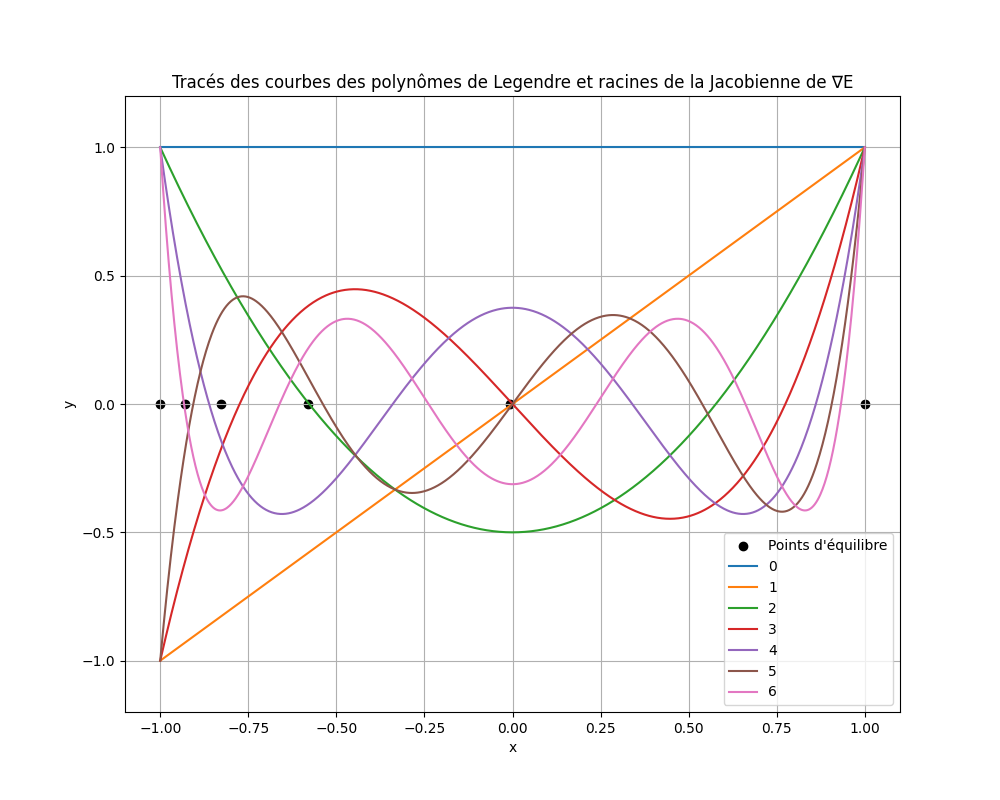
\includegraphics[width=0.65\textwidth]{res/part2_legendre.png}
    \caption{Représentation des courbes des polynômes de Legendre et des racines de la Jacobienne de $\nabla$E}
    \label{fig:p2-c-legendre}
\end{figure} 
On peut constater de manière graphique, sur la Figure \ref{fig:p2-c-legendre}, que la majorité des racines trouvées ressemblent
aux racines des dérivées des polynômes de Legendre. En effet, on peut voir qu'une des racines obtenues est proche de 0
tout comme l'est la racine des dérivées des polynômes de Legendre de degré impair, c'est-à-dire, de degré 1,3 et 5.
La racine proche de -0.58 est aussi proche de celle de la dérivée du polynôme de Legendre de degré 2.
Enfin, celle proche de -0.93 est proche de celle de la dérivée du polynôme de Legendre de degré 6.
\subsection{Maximum ou minimum de l'énergie électrostatique}
Enfin, nous avons cherché à savoir si les solutions correspondent à un maximum ou à un minimum de l'énergie électrostatique.
Pour cela, nous avons tracé l'énergie électrostatique en fonction de la position de la particule, x, ce que l'on peut 
voir sur la Figure \ref{fig:p2-c-2}. En effet, nous avons calculé E(x) pour des x allant de -1 à 1. 
\begin{figure}[htbp!]
    \centering
    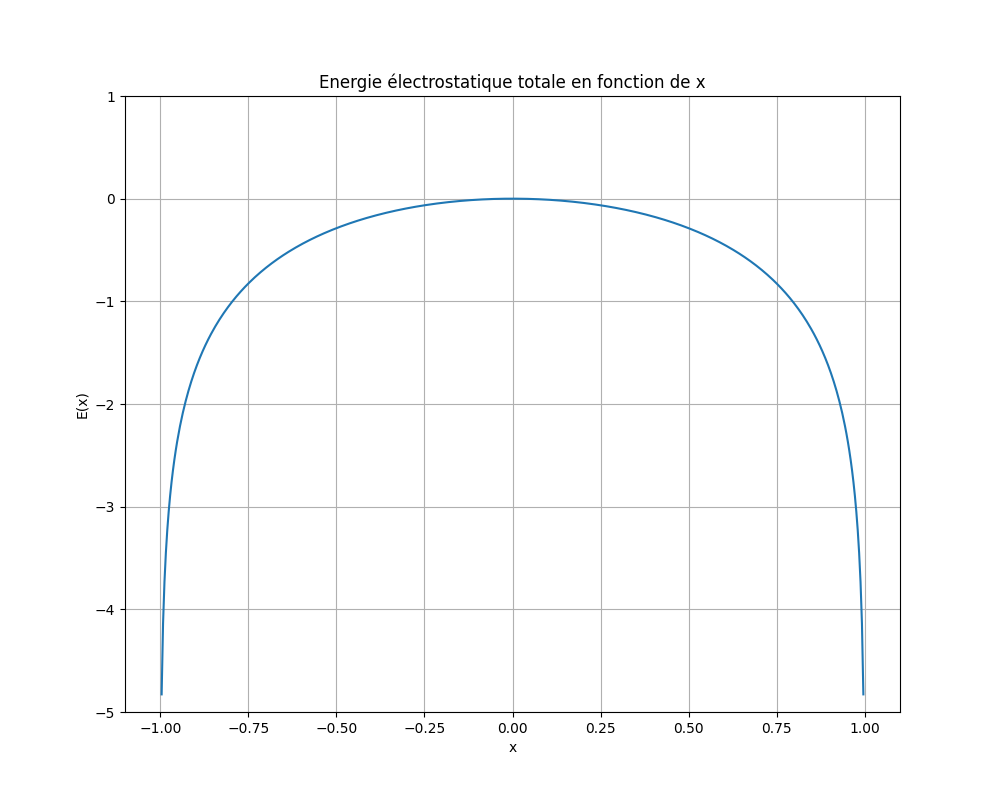
\includegraphics[width=0.65\textwidth]{res/part2_max_min.png}
    \caption{Graphe de l'Energie électrostatique totale en fonction de x}
    \label{fig:p2-c-2}
\end{figure} 
On peut voir sur la Figure \ref{fig:p2-c-2} que les solutions correspondent à un maximum de l'énergie électrostatique. 
En effet, le maximum est atteint en 0 sur le graphe.\label{sec3}

\end{document}